\documentclass{scrartcl}
\usepackage{tikz}
\usetikzlibrary{arrows,automata}
\usepackage{comment}
\usepackage[linguistics]{forest}
\usepackage{textcomp}
\usepackage{makecell}
\usetikzlibrary{automata,positioning}
\usepackage{amsmath,amsfonts,amssymb}
\newcommand{\bl}{{\sqcup}}
\begin{document}
\hfuzz=\maxdimen
\tolerance=10000
\hbadness=10000
\begin{center}
Wen Liang(\texttt{Wen\_Liang@student.uml.edu}) 01724877
\end{center}
\section*{3.1}
\subsection*{a.}
$q_10$,	$\sqcup$$q_2$$\sqcup$, $\sqcup$$\sqcup$$q_{accept}$ 

\subsection*{c.}
$q_1$000, $\sqcup$$q_2$00, $\sqcup$x$q_3$0, $\sqcup$x0$q_4$$\sqcup$, $\sqcup$x0$\sqcup$$q_{reject}$

\subsection*{d.}
$q_1$000000, $\sqcup$$q_2$00000, $\sqcup$x$q_3$0000, $\sqcup$x0$q_4$000,
$\sqcup$x0x$q_3$00, $\sqcup$x0x0$q_4$0, $\sqcup$x0x0x$q_3$$\sqcup$, $\sqcup$x0x0$q_5$x$\sqcup$, $\sqcup$x0x$q_5$0x$\sqcup$, $\sqcup$x0$q_5$x0x$\sqcup$, $\sqcup$x$q_5$0x0x$\sqcup$, $\sqcup$$q_5$x0x0x$\sqcup$, $q_5$$\sqcup$x0x0x$\sqcup$, $\sqcup$$q_2$x0x0x$\sqcup$, $\sqcup$x$q_2$0x0x$\sqcup$, $\sqcup$xx$q_3$x0x$\sqcup$, $\sqcup$xxx$q_3$0x$\sqcup$,
$\sqcup$xxx0$q_4$x$\sqcup$, $\sqcup$xxx0x$q_4$$\sqcup$, $\sqcup$xxx0x$\sqcup$$q_{reject}$
\subsection*{00000000}
$q_100000000\to \bl q_20000000\to \bl xq_3000000\to \bl x0q_400000\to \bl x0xq_30000\to
\bl x0x0q_4000\to \bl x0x0xq_300\to \bl x0x0x0q_40\to \bl x0x0x0xq_3\bl\to \bl x0x0x0q_5x\bl\to \bl x0x0xq_50x\bl\to \bl x0x0q_5x0x\bl\to \bl x0xq_50x0x\bl\to
\bl x0q_5x0x0x\bl\to \bl xq_50x0x0x\bl\to \bl q_5x0x0x0x\bl\to q_5\bl x0x0x0x\bl\to
\bl q_2x0x0x0x\bl\to \bl xq_20x0x0x\bl\to \bl xxq_3x0x0x\bl\to \bl xxxq_30x0x\bl
\to \bl xxx0q_4x0x\bl\to \bl xxx0xq_40x\bl\to \bl xxx0xxq_3x\bl\to \bl xxx0xxxq_3\bl\to \bl xxx0xxq_5x\bl\to \bl xxx0xq_5xx\bl\to \bl xxx0q_5xxx\bl
\to \bl xxxq_50xxx\bl\to \bl xxq_5x0xxx\bl\to \bl xq_5xx0xxx\bl\to \bl q_5xxx0xxx\bl\to q_5\bl xxx0xxx\bl\to \bl q_2xxx0xxx\bl\to \bl xq_2xx0xxx\bl\to \bl xxq_2x0xxx\bl\to \bl xxxq_20xxx\bl\to \bl xxxxq_3xxx\bl\to \bl xxxxxq_3xx\bl
\to \bl xxxxxxq_3x\bl\to \bl xxxxxxxq_3\bl\to \bl xxxxxxq_5x\bl\to \bl xxxxxq_5xx\bl\to \bl xxxxq_5xxx\bl\to \bl xxxq_5xxxx\bl\to \bl xxq_5xxxxx\bl\to \bl xq_5xxxxxx\bl\to \bl q_5xxxxxxx\bl\to q_5\bl xxxxxxx\bl\to \bl q_2xxxxxxx\bl\to \bl xq_2xxxxxx\bl\to \bl xxq_2xxxxx\bl\to \bl xxxq_2xxxx\bl\to \bl xxxxq_2xxx\bl\to \bl xxxxxq_2xx\bl\to \bl xxxxxxq_2x\bl\to \bl xxxxxxxq_2\bl
\to \bl xxxxxxx\bl q_{accept} $

\section*{3.2}

\begin{enumerate}
	
	\item[b.]1\#1. \qquad $q_1 1\#1 \to xq_3 \# 1 \to x\# q_5 1 \to xq_6 \#x \to q_7 x \# x \to xq_1 \# x \to x\#q_8 x \to x\#q_8 \bl \to x\#x{\bl}q_{accept}  $.
	\item[c.]1\#\#1. \qquad $q_1 1\#\#1 \to xq_3 \#\#1 \to x\#q_5\#1 \to x\#\#q_{reject}1$.
	\item[d.]10\#11. \qquad $q_1 10\#11 \to xq_30\#11 \to x0q_3\#11 \to x0\#q_511 \to x0q_6\#x1 \to xq_7 0 \#x1 \to q_7 x 0\#x1 \to xq_1 0 \#x1 \to xxq_2\#x1 \to xx\#q_4 x1 \to xx\#xq_4 1\to xx\#x1q_{reject} \bl $.
	\item[e.]10\#10. \qquad $q_1 10\#10 \to xq_30\#10 \to x0q_3\#10 \to x0\#q_510 \to x0q_6\#x0 \to xq_70\#x0 \to q_7x0\#x0 \to xq_10\#x0 \to xxq_2\#x0 \to xx\#q_4x0 \to xx\#xq_40 \to xx\#q_6xx \to xxq_6\#xx \to xq_7x\#xx \to xq_7x\#xx \to xxq_1\#xx \to xx\#q_8 xx \to xx\#xq_8 x \to xx\#xxq_8 \bl \to xx\#xx \bl q_{accept}  $.
\end{enumerate}

\subsection*{01100\#01100}
$q_1 01100\#01100 \to xq_2 1100\#01100 \to x1q_2100\#01100 \to x11q_200\#01100
\to x110q_20\#01100 \to x1100q_2\#01100 \to x1100\#q_401100 \to x1100q_6\#x1100
\to x110q_70\#x1100 \to x11q_700\#x1100 \to x1q_7100\#x1100 \to xq_71100\#x1100
\to q_7x1100\#x1100 \to xq_11100\#x1100 \to xxq_3100\#x1100 \to xx1q_300\#x1100
\to xx10q_30\#x1100 \to xx100q_3\#x1100 \to xx100\#q_5x1100 \to xx100\#xq_51100
\to xx100\#q_6xx100 \to xx100q_6\#xx100 \to xx10q_70\#xx100 \to xx1q_700\#xx100
\to xxq_7100\#xx100 \to xq_7x100\#xx100 \to xxq_1100\#xx100 \to xxxq_300\#xx100
\to xxx0q_30\#xx100 \to xxx00q_3\#xx100 \to xxx00\#q_5xx100 \to xxx00\#xq_5x100
\to xxx00\#xxq_5100 \to xxx00\#xq_6xx00 \to xxx00\#q_6xxx00 \to xxx00q_6\#xxx00
\to xxx0q_70\#xxx00 \to xxxq_700\#xxx00 \to xxq_7x00\#xxx00 \to xxxq_100\#xxx00
\to xxxxq_20\#xxx00 \to xxxx0q_2\#xxx00 \to xxxx0\#q_4xxx00 \to xxxx0\#xq_4xx00
\to xxxx0\#xxq_4x00 \to xxxx0\#xxxq_400 \to xxxx0\#xxq_6xx0 \to xxxx0\#xq_6xxx0
\to xxxx0\#q_6xxxx0 \to xxxx0q_6\#xxxx0 \to xxxxq_70\#xxxx0 \to xxxq_7x0\#xxxx0
\to xxxxq_10\#xxxx0 \to xxxxxq_2\#xxxx0 \to xxxxx\#q_4xxxx0 \to xxxxx\#xq_4xxx0
\to xxxxx\#xxq_4xx0 \to xxxxx\#xxxq_4x0 \to xxxxx\#xxxxq_40 \to xxxxx\#xxxq_6xx
\to xxxxx\#xxq_6xxx \to xxxxx\#xq_6xxxx \to xxxxx\#q_6xxxxx \to xxxxxq_6\#xxxxx
\to xxxxq_7x\#xxxxx \to xxxxxq_1\#xxxxx \to xxxxx\#q_8xxxxx \to xxxxx\#xq_8xxxx
\to xxxxx\#xxq_8xxx \to xxxxx\#xxxq_8xx \to xxxxx\#xxxxq_8x \to xxxxx\#xxxxxq_8\bl
\to xxxxx\#xxxxx\bl q_{acccept} $

\subsection*{01101\#01100}
$q_1 01101\#01100 \to xq_2 1101\#01100 \to x1q_2101\#01100 \to x11q_201\#01100
\to x110q_21\#01100 \to x1101q_2\#01100 \to x1101\#q_401100 \to x1101q_6\#x1100
\to x110q_71\#x1100 \to x11q_701\#x1100 \to x1q_7101\#x1100 \to xq_71101\#x1100
\to q_7x1101\#x1100 \to xq_11101\#x1100 \to xxq_3101\#x1100 \to xx1q_301\#x1100
\to xx10q_31\#x1100 \to xx101q_3\#x1100 \to xx101\#q_5x1100 \to xx101\#xq_51100
\to xx101\#q_6xx100 \to xx101q_6\#xx100 \to xx10q_71\#xx100 \to xx1q_701\#xx100
\to xxq_7101\#xx100 \to xq_7x101\#xx100 \to xxq_1101\#xx100 \to xxxq_301\#xx100
\to xxx0q_31\#xx100 \to xxx01q_3\#xx100 \to xxx01\#q_5xx100 \to xxx01\#xq_5x100
\to xxx01\#xxq_5100 \to xxx01\#xq_6xx00 \to xxx01\#q_6xxx00 \to xxx01q_6\#xxx00
\to xxx0q_71\#xxx00 \to xxxq_701\#xxx00 \to xxq_7x01\#xxx00 \to xxxq_101\#xxx00
\to xxxxq_21\#xxx00 \to xxxx1q_2\#xxx00 \to xxxx1\#q_4xxx00 \to xxxx1\#xq_4xx00
\to xxxx1\#xxq_4x00 \to xxxx1\#xxxq_400 \to xxxx1\#xxq_6xx0 \to xxxx1\#xq_6xxx0
\to xxxx1\#q_6xxxx0 \to xxxx1q_6\#xxxx0 \to xxxxq_71\#xxxx0 \to xxxq_7x1\#xxxx0
\to xxxxq_11\#xxxx0 \to xxxxxq_3\#xxxx0 \to xxxxx\#q_5xxxx0 \to xxxxx\#xq_5xxx0
\to xxxxx\#xxq_5xx0 \to xxxxx\#xxxq_5x0 \to xxxxx\#xxxxq_50 \to xxxxx\#xxxxq_{reject}0$

\section*{3.8}
\subsection*{b}
1. Scan the tape and mark the first 1 which has not been marked. If no unmarked 1’s are
found go to stage 5. Otherwise move the head back to the start of the tape\\
2. Scan the tape until an unmarked 0 is found, mark the 0, if no 0’s are found reject\\
3. Scan the tape once more until an unmarked zero is found, mark the 0, if no 0’s are found
reject\\
4. Move the head back to the start of the tape and go to stage 1\\
5. Move the head back to the start of the tape. Scan the tape to see if any unmarked 0’s are
found. If none are found accept, otherwise reject.
\begin{tikzpicture}[>=stealth',shorten >=1pt,auto,node distance=2.7cm]


\node[initial,state	]   (q1)      				{$q_1$};
\node[state] 	  (q2) [right of=q1]  	{$q_2$};
\node[state] 	  (q3) [right of=q2]  	{$q_3$};
\node[state] 	  (q4) [right of=q3]  	{$q_4$};
\node[state] 	  (q5) [right of=q4]  	{$q_5$};
\node[state] 	  (q6) [right of=q5]  	{$q_6$};
\node[state] 	  (q7) [above of=q5]  	{$q_7$};
\node[state] 	  (q8) [above of=q7]  	{$q_8$};
\node[state] 	  (q9) [above of=q8]  	{$q_9$};
\node[state] 	  (qa) [above of=q9]  	{$q_{accept}$};
\node[state] 	  (qA) [below of=q1]  	{$q_A$};
\node[state] 	  (qB) [below of=qA]  	{$q_B$};
\node[state] 	  (qC) [below of=qB]  	{$q_C$};
\node[state] 	  (qD) [below of=qC]  	{$q_D$};
\node[state] 	  (qE) [below of=qD]  	{$q_E$};
\node[state] 	  (qF) [right of=qE]  	{$q_F$};
\node[state] 	  (qG) [right of=qF]  	{$q_G$};
\node[state] 	  (qH) [right of=qG]  	{$q_H$};
\node[state] 	  (qI) [right of=qH]  	{$q_I$};
\node[state] 	  (qJ) [right of=qC]  	{$q_J$};
\node[state] 	  (qK) [right of=qJ]  	{$q_K$};
\node[state] 	  (qL) [right of=qK]  	{$q_{accept}$};

\path[->] (q1)  edge	  	node{$1\to\$,R$}	(q2)
edge	  	node{$\bl\to R$}	(qa)
edge	  	node{$0\to\$,R$}	(qA)
(q2)  edge[loop above]	 node{$1,x,y\to R$} 		(q2)

edge  	node{$0\to y, R$}  	(q3)
(q3)  edge[loop above]	 node{$1,x,y\to R$} 		(q3)

edge  	node{$0\to y,L$}  	(q4)
(q4)  edge[loop above]	 node{$1,x,y\to L$} 		(q4)
		edge	 node{$ \$\to R$} 		(q5)
(q5)  edge[loop below]	 node{$0,x,y\to R$} 		(q5)
edge	 node{$1\to x, L$} 		(q6)
edge	 node{$\bl\to L$} 		(q7)
(q6)  edge[loop above]	 node{$0,x,y\to L$} 		(q6)
edge[bend left]	 node{$\$\to R$} 		(q2)
(q7)  edge[loop right]	 node{$0,x,y\to L$} 		(q7)
edge	 node{$\$\to R$} 		(q8)
(q8)  edge	 node{$x,y\to R$} 		(q9)
(q9)  edge	 node{$\bl\to R$} 		(qa)
(qA)  edge[loop right]	 node{$1\to R$} 		(qA)
edge	 node{$0\to y,L$} 		(qB)
(qB)  edge[loop right]	 node{$1\to L$} 		(qB)
edge	 node{$\$\to R$} 		(qC)
(qC)  edge[loop left]	 node{$0,x,y\to R$} 		(qC)
edge[left]	 node{$1\to x,L$} 		(qD)
(qD)  edge[loop left]	 node{$0,x,y\to L$} 		(qD)
edge[left]	 node{$\$\to R$} 		(qE)
(qE)  edge[loop left]	 node{$0,x,y\to R$} 		(qE)
edge	 node{$1\to x,L$} 		(qF)
edge[right]	 node{$\bl\to L$} 		(qJ)
(qF)  edge[loop above]	 node{$0,x,y\to L$} 		(qF)
edge	 node{$\$\to R$} 		(qG)

(qG)  edge[loop above]	 node{$1,x,y\to R$} 		(qG)
edge	 node{$0\to y, R$} 		(qH)
(qH)  edge[loop above]	 node{$1,x\to R$} 		(qH)
edge	 node{$0\to y, L$} 		(qI)
(qI)  edge[loop right]	 node{$1,x,y\to L$} 		(qI)
edge[bend right=60]	 node{$\$\to R$} 		(qE)
(qJ)  edge[loop above]	 node{$0,x,y\to L$} 		(qJ)
edge	 node{$\$\to R$} 		(qK)
(qK)  edge[loop above]	 node{$x,y\to R$} 		(qK)
edge	 node{$\bl\to R$} 		(qL);
\end{tikzpicture}
\section*{Note: Because the space of the page, I can not lable the transition to the reject state, all the input string can not reach the accept state or stuck in some state because of the next input symbol can not match the transition function here will directly go to the reject state,aka $q_{reject}$.} 
\subsection*{010100}
$q_1010100\to\$q_A10100\to\$1q_A0100\to\$q_B1y100\to q_B\$1y100\to\$q_C1y100 \to\$q_Dxy100\to q_D\$xy100\to\$q_Exy100\to\$xq_Ey100\to\$xyq_E100\to\$xq_Fyx00
\to\$q_Fxyx00\to q_F\$xyx00\to\$q_Gxyx00\to\$xq_Gyx00\to\$xyq_Gx00\to\$xyxq_G00
\to\$xyxyq_H0\to\$xyxq_Iyy\to\$xyq_Ixyy\to\$xq_Iyxyy\to\$q_Ixyxyy\to q_I\$xyxyy
\to\$q_Exyxyy\to\$xq_Eyxyy\to\$xyq_Exyy\to\$xyxq_Eyy\to\$xyxyq_Ey\to\$xyxyyq_E\bl
\to\$xyxyq_Jy\bl\to\$xyxq_Jyy\bl\to\$xyq_Jxyy\bl\to\$xq_Jyxyy\bl\to\$q_Jxyxyy\bl
\to q_J\$xyxyy\bl\to\$ q_Kxyxyy\bl\to\$xq_Kyxyy\bl\to\$xyq_Kxyy\bl\to\$xyxq_Kyy\bl
\to\$xyxyq_Ky\bl\to\$xyxyyq_K\bl\to\$xyxyy\bl q_{accept}$

\subsection*{010101}
$q_1010101\to\$q_A10101\to\$1q_A0101\to\$q_B1y101\to q_B\$1y101\to\$q_C1y101 \to\$q_Dxy101\to q_D\$xy101\to\$q_Exy101\to\$xq_Ey101\to\$xyq_E101\to\$xq_Fyx01
\to\$q_Fxyx01\to q_F\$xyx01\to\$q_Gxyx01\to\$xq_Gyx01\to\$xyq_Gx01\to\$xyxq_G01
\to\$xyxyq_H1\to\$xyxy1q_H\bl\to\$xyxy1q_{reject}\bl$
\subsection*{c}
1. Scan the tape and mark the first 1 which has not been marked. If no unmarked 1’s are
found go to stage 5. Otherwise move the head back to the start of the tape\\
2. Scan the tape until an unmarked 0 is found, mark the 0, if no 0’s are found accept\\
3. Scan the tape once more until an unmarked zero is found, mark the 0, if no 0’s are found
accept\\
4. Move the head back to the start of the tape and go to stage 1\\
5. Move the head back to the start of the tape. Scan the tape to see if any unmarked 0’s are
found. If none are found reject, otherwise accept

\begin{tikzpicture}[>=stealth',shorten >=1pt,auto,node distance=2.7cm]


\node[initial,state	]   (q1)      				{$q_1$};
\node[state] 	  (q2) [right of=q1]  	{$q_2$};
\node[state] 	  (q3) [right of=q2]  	{$q_3$};
\node[state] 	  (q4) [right of=q3]  	{$q_4$};
\node[state] 	  (q5) [right of=q4]  	{$q_5$};
\node[state] 	  (q6) [right of=q5]  	{$q_6$};
\node[state] 	  (q7) [above of=q5]  	{$q_7$};
\node[state] 	  (q8) [above of=q7]  	{$q_8$};
\node[state] 	  (q9) [above of=q8]  	{$q_9$};
\node[state] 	  (qa) [above of=q9]  	{$q_{reject}$};
\node[state] 	  (qA) [below of=q1]  	{$q_A$};
\node[state] 	  (qB) [below of=qA]  	{$q_B$};
\node[state] 	  (qC) [below of=qB]  	{$q_C$};
\node[state] 	  (qD) [below of=qC]  	{$q_D$};
\node[state] 	  (qE) [below of=qD]  	{$q_E$};
\node[state] 	  (qF) [right of=qE]  	{$q_F$};
\node[state] 	  (qG) [right of=qF]  	{$q_G$};
\node[state] 	  (qH) [right of=qG]  	{$q_H$};
\node[state] 	  (qI) [right of=qH]  	{$q_I$};
\node[state] 	  (qJ) [right of=qC]  	{$q_J$};
\node[state] 	  (qK) [right of=qJ]  	{$q_K$};
\node[state] 	  (qL) [right of=qK]  	{$q_{reject}$};

\path[->] (q1)  edge	  	node{$1\to\$,R$}	(q2)
edge	  	node{$\bl\to R$}	(qa)
edge	  	node{$0\to\$,R$}	(qA)
(q2)  edge[loop above]	 node{$1,x,y\to R$} 		(q2)

edge  	node{$0\to y, R$}  	(q3)
(q3)  edge[loop above]	 node{$1,x,y\to R$} 		(q3)

edge  	node{$0\to y,L$}  	(q4)
(q4)  edge[loop above]	 node{$1,x,y\to L$} 		(q4)
edge	 node{$ \$\to R$} 		(q5)
(q5)  edge[loop below]	 node{$0,x,y\to R$} 		(q5)
edge	 node{$1\to x, L$} 		(q6)
edge	 node{$\bl\to L$} 		(q7)
(q6)  edge[loop above]	 node{$0,x,y\to L$} 		(q6)
edge[bend left]	 node{$\$\to R$} 		(q2)
(q7)  edge[loop right]	 node{$0,x,y\to L$} 		(q7)
edge	 node{$\$\to R$} 		(q8)
(q8)  edge	 node{$x,y\to R$} 		(q9)
(q9)  edge	 node{$\bl\to R$} 		(qa)
(qA)  edge[loop right]	 node{$1\to R$} 		(qA)
edge	 node{$0\to y,L$} 		(qB)
(qB)  edge[loop right]	 node{$1\to L$} 		(qB)
edge	 node{$\$\to R$} 		(qC)
(qC)  edge[loop left]	 node{$0,x,y\to R$} 		(qC)
edge[left]	 node{$1\to x,L$} 		(qD)
(qD)  edge[loop left]	 node{$0,x,y\to L$} 		(qD)
edge[left]	 node{$\$\to R$} 		(qE)
(qE)  edge[loop left]	 node{$0,x,y\to R$} 		(qE)
edge	 node{$1\to x,L$} 		(qF)
edge[right]	 node{$\bl\to L$} 		(qJ)
(qF)  edge[loop above]	 node{$0,x,y\to L$} 		(qF)
edge	 node{$\$\to R$} 		(qG)

(qG)  edge[loop above]	 node{$1,x,y\to R$} 		(qG)
edge	 node{$0\to y, R$} 		(qH)
(qH)  edge[loop above]	 node{$1,x\to R$} 		(qH)
edge	 node{$0\to y, L$} 		(qI)
(qI)  edge[loop right]	 node{$1,x,y\to L$} 		(qI)
edge[bend right=60]	 node{$\$\to R$} 		(qE)
(qJ)  edge[loop above]	 node{$0,x,y\to L$} 		(qJ)
edge	 node{$\$\to R$} 		(qK)
(qK)  edge[loop above]	 node{$x,y\to R$} 		(qK)
edge	 node{$\bl\to R$} 		(qL);
\end{tikzpicture}

\section*{Note: Because the space of the page, I can not lable the transition to the accept state, all the input string can not reach the reject state or stuck in some state because of the next input symbol can not match the transition function here will directly go to the accept state,aka $q_{accept}$.} 
\subsection*{000111}
$q_1000111\to\$q_A00111\to q_B\$y0111\to\$q_Cy0111\to\$yq_C0111\to\$y0q_C111
\to\$yq_D0x11\to\$q_Dy0x11\to q_D\$y0x11\to\$q_Ey0x11\to\$yq_E0x11\to\$y0q_Ex11
\to\$y0xq_E11\to\$y0q_Fxx1\to\$yq_F0xx1\to\$q_Fy0xx1\to q_F\$y0xx1\to \$q_Gy0xx1
\to \$yq_G0xx1\to\$yyq_Hxx1\to\$yyxq_Hx1\to\$yyxxq_H1\to\$yyxx1q_H\bl
\to\$yyxx1\bl q_{accept}$


\subsection*{000110}
$q_1000110\to\$q_A00110\to q_B\$y0110\to\$q_Cy0110\to\$yq_C0110\to\$y0q_C110
\to\$yq_D0x10\to\$q_Dy0x10\to q_D\$y0x10\to\$q_Ey0x10\to\$yq_E0x10\to\$y0q_Ex10
\to\$y0xq_E10\to\$y0q_Fxx0\to\$yq_F0xx0\to\$q_Fy0xx0\to q_F\$y0xx0\to \$q_Gy0xx0
\to \$yq_G0xx0\to\$yyq_Hxx0\to\$yyxq_Hx0\to\$yyxxq_H0\to\$yyxq_Ixy\to\$yyq_Ixxy
\to\$yq_Iyxxy\to\$q_Iyyxxy\to q_I\$yyxxy\to\$q_Eyyxxy\to\$yq_Eyxxy\to\$yyq_Exxy
\to\$yyxq_Exy\to\$yyxxq_Ey\to\$yyxxyq_E\bl\to\$yyxxq_Jy\bl\to\$yyxq_Jxy\bl
\to\$yyq_Jxxy\bl\to\$yq_Jyxxy\bl\to\$q_Jyyxxy\bl\to q_J\$yyxxy\bl\to\$q_Kyyxxy\bl
\to\$yq_Kyxxy\bl\to\$yyq_Kxxy\bl\to\$yyxq_Kxy\bl\to\$yyxxq_Ky\bl\to\$yyxxyq_K\bl
\to\$yyxxy\bl q_{reject}$


\section*{Modify machine M2 to recognize odd number of 0s and draw the state diagram.}

\begin{tikzpicture}[>=stealth',shorten >=1pt,auto,node distance=4cm]


\node[initial,state	]   (q1)      				{$q_1$};
\node[state] 	  (q2) [right of=q1]  	{$q_2$};
\node[state] 	  (q3) [right of=q2]  	{$q_3$};
\node[state] 	  (qa) [below of=q2]  	{$q_{accept}$};
\node[state] 	  (qr) [below of=q3]  	{$q_{reject}$};

\path[->] (q1)  edge	  	node{$0\to \bl,R$}	(q2)


(q2)  edge[bend left]	 node{$0\to x,R$} 		(q3)
	
edge  	node{$\bl\to R$}  	(qa)
(q3)  edge[bend left]	 node{$0\to y,R$} 		(q2)

edge  	node{$\bl\to R$}  	(qr);

\end{tikzpicture}
\subsection*{000}
$q_1000\to \bl q_200\to\bl xq_30\to\bl xyq_2\bl\to\bl xy\bl q_{accept}$
\subsection*{0000}
$q_10000\to \bl q_2000\to\bl xq_300\to\bl xyq_20\to\bl xyxq_3\bl\to\bl xyx\bl q_{reject}$



\section*{Modify machine M2 to recognize even number of 0s and draw the state diagram.}
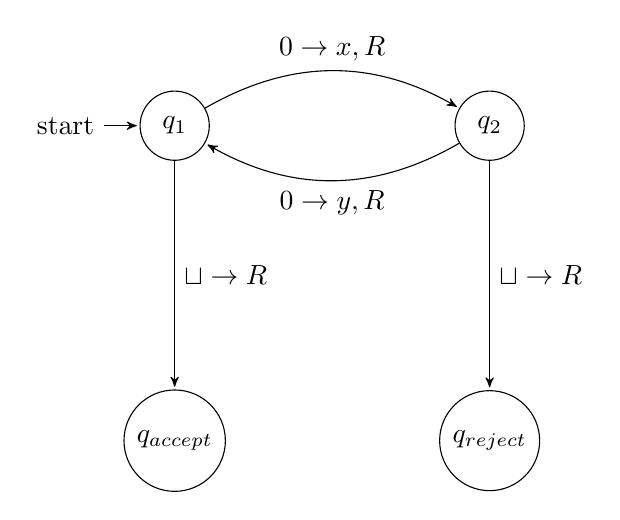
\begin{tikzpicture}[>=stealth',shorten >=1pt,auto,node distance=4cm]


\node[initial,state	]   (q1)      				{$q_1$};
\node[state] 	  (q2) [right of=q1]  	{$q_2$};

\node[state] 	  (qa) [below of=q1]  	{$q_{accept}$};
\node[state] 	  (qr) [below of=q2]  	{$q_{reject}$};

\path[->] (q1)  edge[bend left]	  	node{$0\to x,R$}	(q2)
edge  	node{$\bl\to R$}  	(qa)

(q2)  edge[bend left]	 node{$0\to y,R$} 		(q1)

edge  	node{$\bl\to R$}  	(qr);

\end{tikzpicture}

\subsection*{000}
$q_1000\to xq_200\to xyq_10\to xyxq_2\bl\to xyx\bl q_{reject}$
\subsection*{0000}
$q_10000\to xq_2000\to xyq_100\to xyxq_20\to xyxyq_1\bl\to xyxy\bl q_{accept}$
\end{document}
